\section{Results}
\label{sec:results}
%(Sam Schmidt, Bryce Kalmbach, Johann Cohen Tanugi, Rongpu Zhou)

\subsection{Ensembles of photo-\mathinhead{$z$}{z} interim posteriors}

\begin{figure*}
%\centering
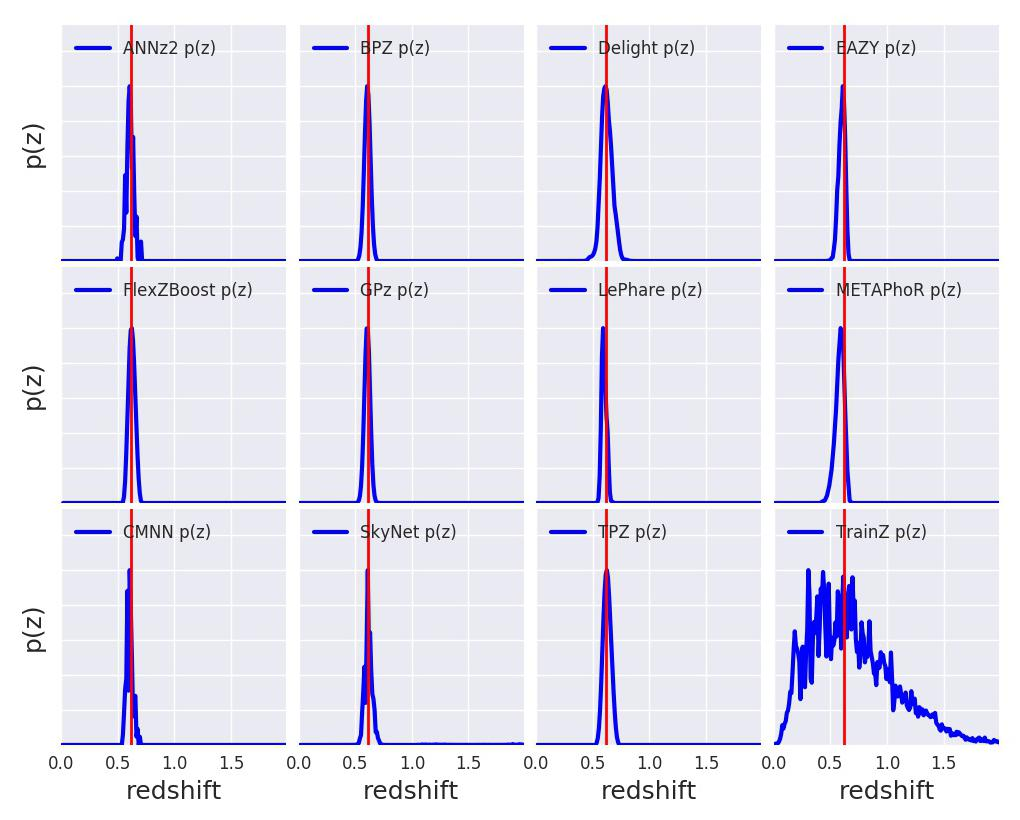
\includegraphics[width=0.49\textwidth]{fig/pz_12codes_261931_crop.jpg}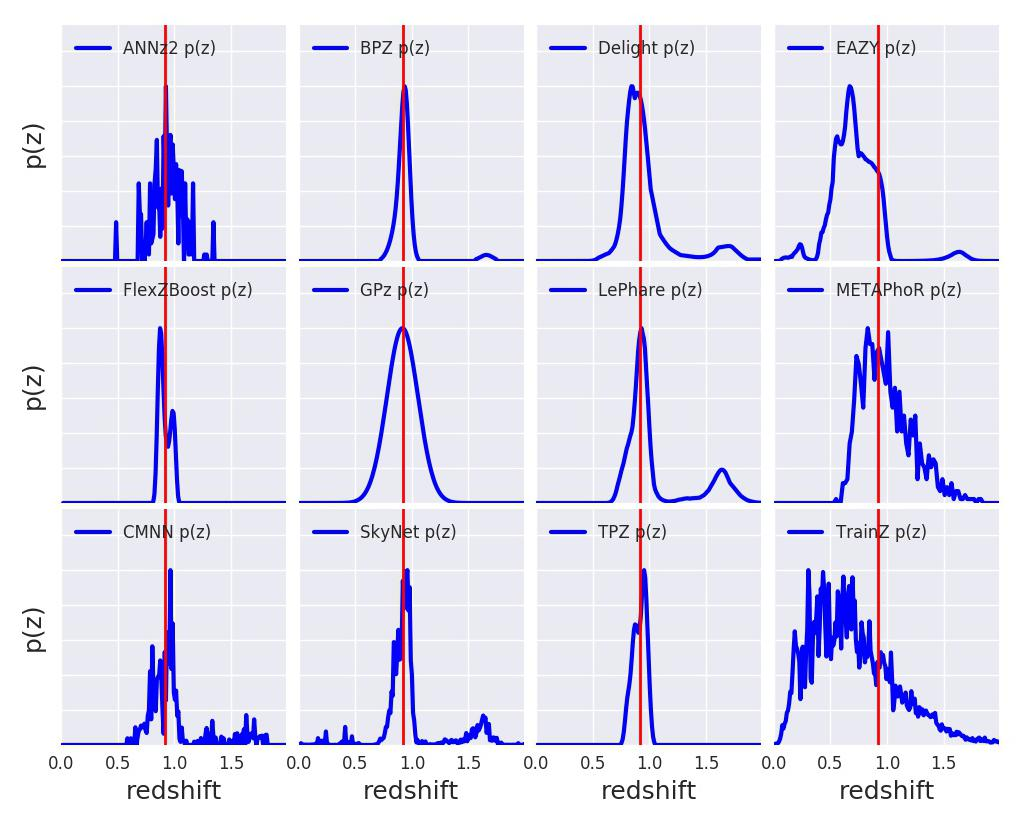
\includegraphics[width=0.5\textwidth]{fig/pz_12codes_471167_crop.jpg}\\
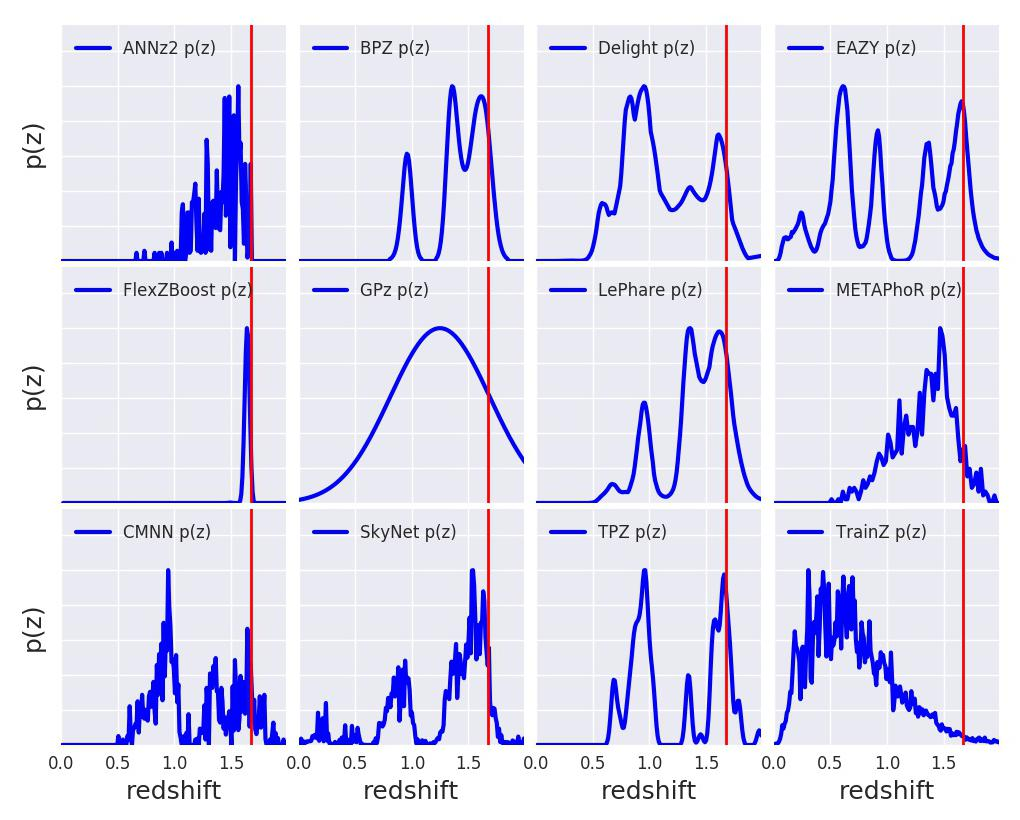
\includegraphics[width=0.49\textwidth]{fig/pz_12codes_713178_crop.jpg}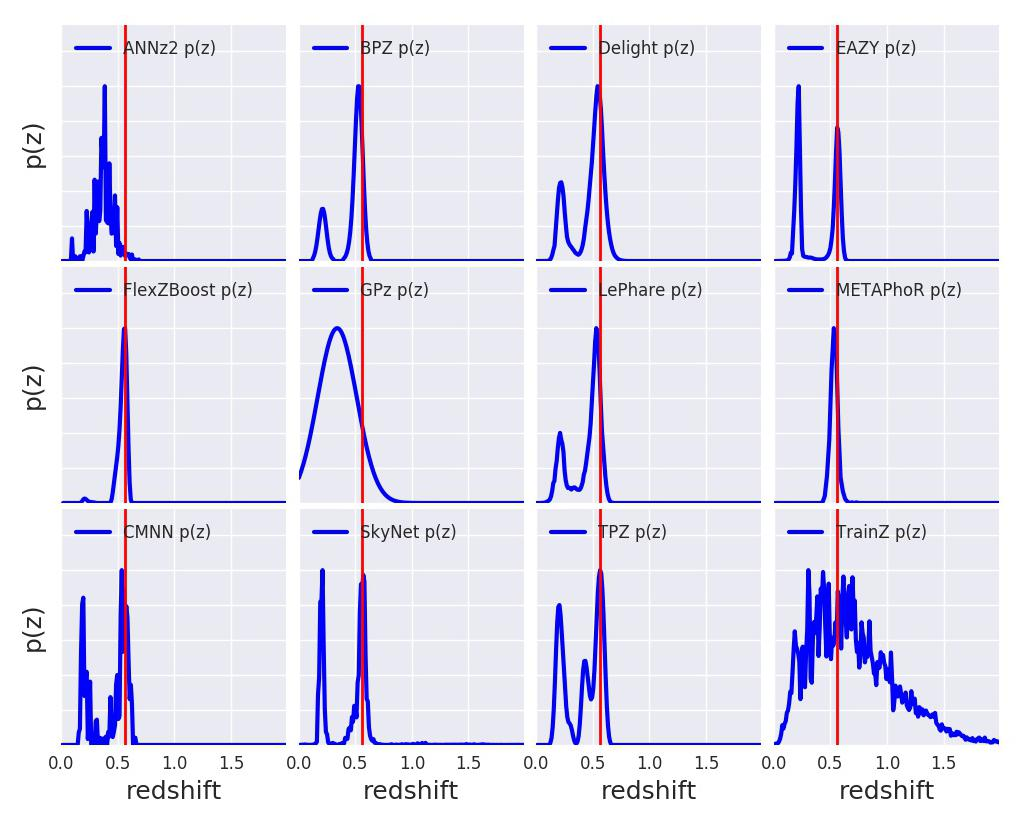
\includegraphics[width=0.49\textwidth]{fig/pz_12codes_982747_crop.jpg}
\caption{Four illustrative examples of individual p(z) distributions produced by the codes.  The red vertical line represents the true redshift.  Examples are chosen with common features seen in PDFs: tight unimodal $p(z)$ (upper left), broad unimodal $p(z)$ (upper right), bimodal $p(z)$ (lower right), and complex/multimodal $p(z)$ (lower left).  Codes show varying amounts of small-scale structure in their reconstruction of the posterior distribution.  We see varying responses from the codes in the presence of color degeneracies and photometric errors, resulting in narrow and broad unimodal, bimodal, and multi-modal $p(z)$ curves.} \label{fig:pz_examples}
\end{figure*}

%\begin{figure*}
%\centering
%\includegraphics[width=\textwidth]{fig/QQplot_11codes.jpg}
%\caption{The QQ plots produced for every photo-$z$ code.  \aim{Consider making this a plot of QQ minus that diagonal for better contrast between methods.}\red{The PIT histogram is essentially this, which is one of the main reasons to include both.  QQ is a fairly standard form, so plotting in this fashion rather than the difference seems better to me, given that we also ahve the PIT histograms. --SJS}} \label{fig:qq}
%\end{figure*}

\begin{figure*}
\centering
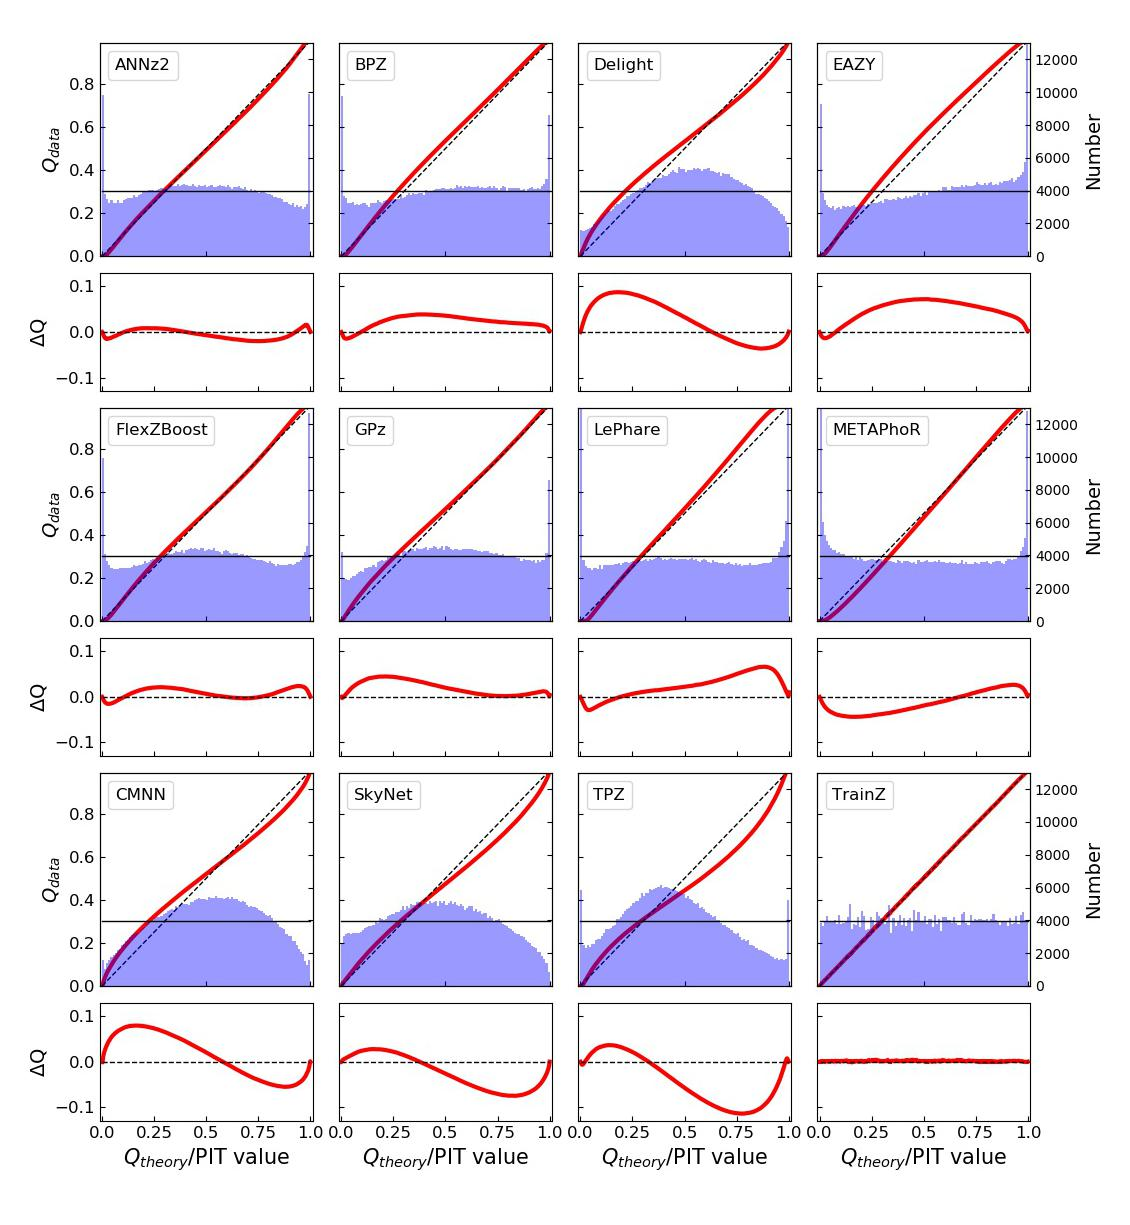
\includegraphics[width=\textwidth]{fig/PITANDQQplot_12codes_crop.jpg}
\caption{Summary plots for all twelve photo-$z$ codes illustrating performance for the interim posterior statistics. The top panel of each pair shows both the Quantile-Quantile (QQ) plot (red) and the histogram of PIT values (blue).  The desired behavior is a QQ plot that matches the diagonal dashed line, and a PIT histogram that matches a uniform distribution matching the thin horizontal black line.  The bottom panel of each pair shows the difference between the QQ quantile and the diagonal, illustrating departure from the desired performance.  Histograms with an overabundance of PIT values at the centre of the distribution indicate $p(z)$ distributions that are overly broad, while an excess of values at the extrema indicate $p(z)$ distributions that are overly narrow.  Values of PIT=0 and PIT=1 indicate ``catastrophic failures'' where the true redshift is completely outside the support of $p(z)$.  Asymmetric features are indicative of systematic bias in the redshift predictions.  A variety of behaviors are evident, and specific details are discussed in the text.}
\label{fig:pitqq}
\end{figure*}

Fig.~\ref{fig:pz_examples} Shows the $p(z)$ produced by each of our twelve photo-$z$ codes for four example galaxies which exemplify some prominent cases that arise when estimating photo-$z$ PDFs: a narrow, unimodal redshift solution, a broader unimodal solution, a bimodal distribution, and a complex, multimodal distribution.
The red vertical line represents the true redshift of the individual galaxy, and the blue curve represents the redshift probability.
Several features are obvious even in these illustrative examples.
\textsc{ANNz2, METAPhoR, NN,} and \textsc{SkyNet} all show an excess of small-scale features, which appear to be print-through of the underlying training set galaxies.  For example, in \textsc{CMNN} the $p(z)$ are a simply a weighted histogram of all spectroscopic training galaxies in nearby colour space with no smoothing applied, so the substructure is due to the finite number of neighbours, and is not unexpected.
\textsc{GPZ} (in its current implementation), on the other hand, always produces a single Gaussian, which broadens to cover the multi-modal redshift solutions seen in other codes.
%Interestingly, while \textsc{ANNz2} shows an abundance of small scale structure in individual $p(z)$ measurements (see Fig.~\ref{fig:pz_examples}), the summed $\hat{N}(z)$ is rather smooth, where the small scale features average out.  This is not the case for the two other codes that show an abundance of substructure in their individual $p(z)$: both \textsc{CMNN} and \textsc{SkyNet} show small scale features both in $p(z)$ and $\hat{N}(z)$.

As stated in Section~\ref{sec:metrics}, $p(z)$ is parameterized as $\approx 200$ piecewise constant bins covering $0<z<2$ for all twelve codes, giving a grid size of roughly $\delta z = 0.01$ for each code.
A piecewise constant grid was a natural choice for some photo-$z$ codes, for instance most template-based codes compute likelihoods on a fixed grid.
In contrast, FlexZBoost, for example, can return estimates on any grid without compression errors as it’s a basis expansion method where only the expansion coefficients need to be stored.
Codes with a native output format other than the shared piecewise constant binning scheme (or one that can be losslessly converted to it) may suffer from loss of information when converting to it, which could artificially favor some codes over others.

Furthermore, the fidelity of photo-$z$ interim posteriors in this format varies with the quality of the photometry.
For faint galaxies, this redshift resolution is sufficient to capture the shape of $p(z)$ for the majority of the test sample, where photometric errors on the faint galaxies lead to somewhat broad peaks in the redshift posterior.
However, as can be seen in e.~g.~the top left panel of Fig.~\ref{fig:pz_examples}, for bright galaxies with narrow $p(z)$ the grid spacing of $\delta z = 0.01$ is not sufficient to resolve the peak.
This is consistent with the results described in \citet[]{Malz:qp}, who find that quantiles (and, to a lesser degree, samples) often outperform gridded $p(z)$, particularly for bright objects and in the presence of harsher storage constraints.
With a full 200 numbers to capture the information of each photo-$z$ PDF, any parametrization will perform adequately, but other storage parametrizations and limits on storage resources may be considered in future work.
%Switching to a quantile based parameterization may be more costly computationally, for example template-based codes would need to test more grid point in order to resolve the quantiles for bright galaxies.  However, the computational time for template based codes scales roughly linearly with the number of grid points, so this may be a reasonable thing to implement.
We will discuss this further in Section~\ref{sec:discussion}.
% \red{someone review this statement to make sure that I'm saying this correctly!}

Fig.~\ref{fig:pitqq} shows both the quantile-quantile plots (red) and the histogram of PIT values (blue) summarizing the results from each photo-$z$ code.  The red line shows the measured quantiles, while the black diagonal represents the ideal QQ values if the distribution were perfectly reproduced.  A second panel below the main panel for each code shows the difference between $Q_{data}$ and $Q_{theory}$, i.~e.~the departure from the diagonal, for clarity.
Biases and trends in whether the average width of the $p(z)$ values being over/under-predicted are evident.  An overall bias where the predicted redshift is systematically low manifests as the measured QQ value falling above the diagonal, as is the case for \textsc{BPZ} and \textsc{EAZY}, while a systematic overprediction shows up as the measured QQ value falling below the diagonal, as seen in \textsc{TPZ}.  In terms of PIT histograms, a systematic underprediction of redshift corresponds to fewer PIT values at $PIT<0.5$ and more at $PIT>0.5$, while a systematic overprediction will show the opposite.

Examination of the PIT histograms and QQ plots shows that there are fairly generic issues with the width of $p(z)$ uncertainties: \textsc{Delight, CMNN, SkyNet} and \textsc{TPZ} all show a PIT histogram with an dearth of low values and and an excess of high values, signs that, on average, their $p(z)$ are more broad than the true distribution of redshifts.  \textsc{METAPhoR} shows the opposite trend, indicating the the $p(z)$  are more narrow than the distributions given by the true redshifts.  In all of these code cases there is a free parameter or bandwidth that can be used to tune uncertainties.  The sensitivity of multiple codes to this bandwidth choice emphasizes the fact that great care must be taken in setting user-defined parameters in photo-$z$ codes, even in the presence of representative training/validation data.  for \textsc{FlexZBoost} the ``sharpening'' parameter (described in Section~\ref{sec:flexzboost}) plays a key role in improving the results, resulting in a QQ plot that is very nearly diagonal.  A similar sharpening procedure could be beneficial for several codes.
Interestingly, the three purely template-based codes, \textsc{BPZ, EAZY}, and \textsc{LePhare}, show relatively well behaved $p(z)$ statistics (albeit with some bias), which may indicate that the likelihood estimation with representative templates is accurately capturing the uncertainties on individual redshifts.

%Fig.~\ref{fig:pitqq} shows the PIT histogram plots produced by each photo-$z$ code.
%These plots show information that is very similar to that shown in the QQ plot in many ways.
The ideal PIT histogram would follow the black dashed line, representing a uniform distribution of PIT values, equivalent to the diagonal line in the QQ plot.
Overly broad $p(z)$ values show up as an excess of PIT values near $0.5$ and a dearth of values at the edges, while overly narrow $p(z)$ will have an excess at the edges and will be missing values at the centre.
Another feature evident in the PIT histograms is the number of ``catastrophic outlier'' values where the true redshift falls outside of the non-zero support of $p(z)$, corresponding to PIT$=0.0$ or $1.0$ is more apparent than in the QQ plots.  Following Kodra \& Newman (in prep.) we define $f_{\rm O}$ as the fraction of objects with $PIT<0.0001$ or $PIT>0.9999$.  Table~\ref{tab:pitoutlier} lists these fractions for each of the codes. For a proper Uniform distribution we expect a value of $0.0002$.  Several codes show a marked excess, with \textsc{ANNz2, FlexZBoost, LePhare, and METAPhoR} with $f_{\rm O} > 0.02$, indicating a sizeable number of catastrophic redshift solutions where the true redshift is not covered by the extent of $p(z)$.  For \textsc{METAPhoR} this may be partially due to an overall underprediction of the $p(z)$ width, however this is not the case for the other codes.  \textsc{LePhare} is a particular outlier with nearly 5 per cent of objects outside of $p(z)$ support.  Further study will be necessary to determine what is causing these misclassifications for \textsc{LePhare}.  As expected, and by design, \textsc{TrainZ} has the proper fraction of outliers for the $f_{\rm O}$ statistic.


\begin{table}
\setlength{\tabcolsep}{2pt}
\centering
\caption{The fraction of ``catastrophic outlier'' PIT values.  We expect a value of 0.0002 for a proper Uniform distribution.  An excess over this small value indicates true redshifts that fall outside the non-zero support of the $p(z)$.  }\label{tab:pitoutlier}
\begin{tabular}{lc}
\hline
\hline
 ``catastrophic outlier''\\ PIT fraction\\
\hline
Photo-z Code & fraction PIT$<10^{-4}$ or $>$0.9999\\
\hline
\textsc{ANNz2} & 0.0265\\
\textsc{BPZ} & 0.0192\\
\textsc{Delight} & 0.0006\\
\textsc{EAZY} & 0.0154\\
\textsc{FlexZBoost} & 0.0202\\
\textsc{GPz} & 0.0058\\
\textsc{LePhare} & 0.0486\\
\textsc{METAPhoR}& 0.0229\\
\textsc{CMNN} & 0.0034\\
\textsc{Skynet} & 0.0001\\
\textsc{TPZ} & 0.0130\\
\hline
\textsc{TrainZ} & 0.0002\\
\end{tabular}
\end{table}


%\begin{figure*}
%\centering
%\includegraphics[width=\textwidth]{fig/PIT_histogram_plot_11codes.jpg}
%\caption{The PIT histogram plots produced for every photo-$z$ code.  Ideal behaviour would match a uniform distribution, indicated by the horizontal dashed line.  Histograms with an overabundance of PIT values at the centre of the distribution indicate $p(z)$ distributions that are overly broad, while an excess of values at the extrema indicate $p(z)$ distributions that are overly narrow.  Values of PIT=0 and PIT=1 indicate ``catastrophic failures'' where the true redshift is completely outside the support of $p(z)$.  Asymmetric features are indicative of systematic bias in the redshift predictions.
%\aim{Could we combine this with the previous figure by plotting both as differences from ideal on one plot with left and right axis labels?  The information seems degenerate (which makes sense!)}\red{as you say, the information is degenerat, this form emphasizes the differences a bit more, and shows off the catastrophic outliers with PIT=0 and 1 a bit better in my mind.} } \label{fig:pit}
%\end{figure*}
\begin{figure*}
\centering
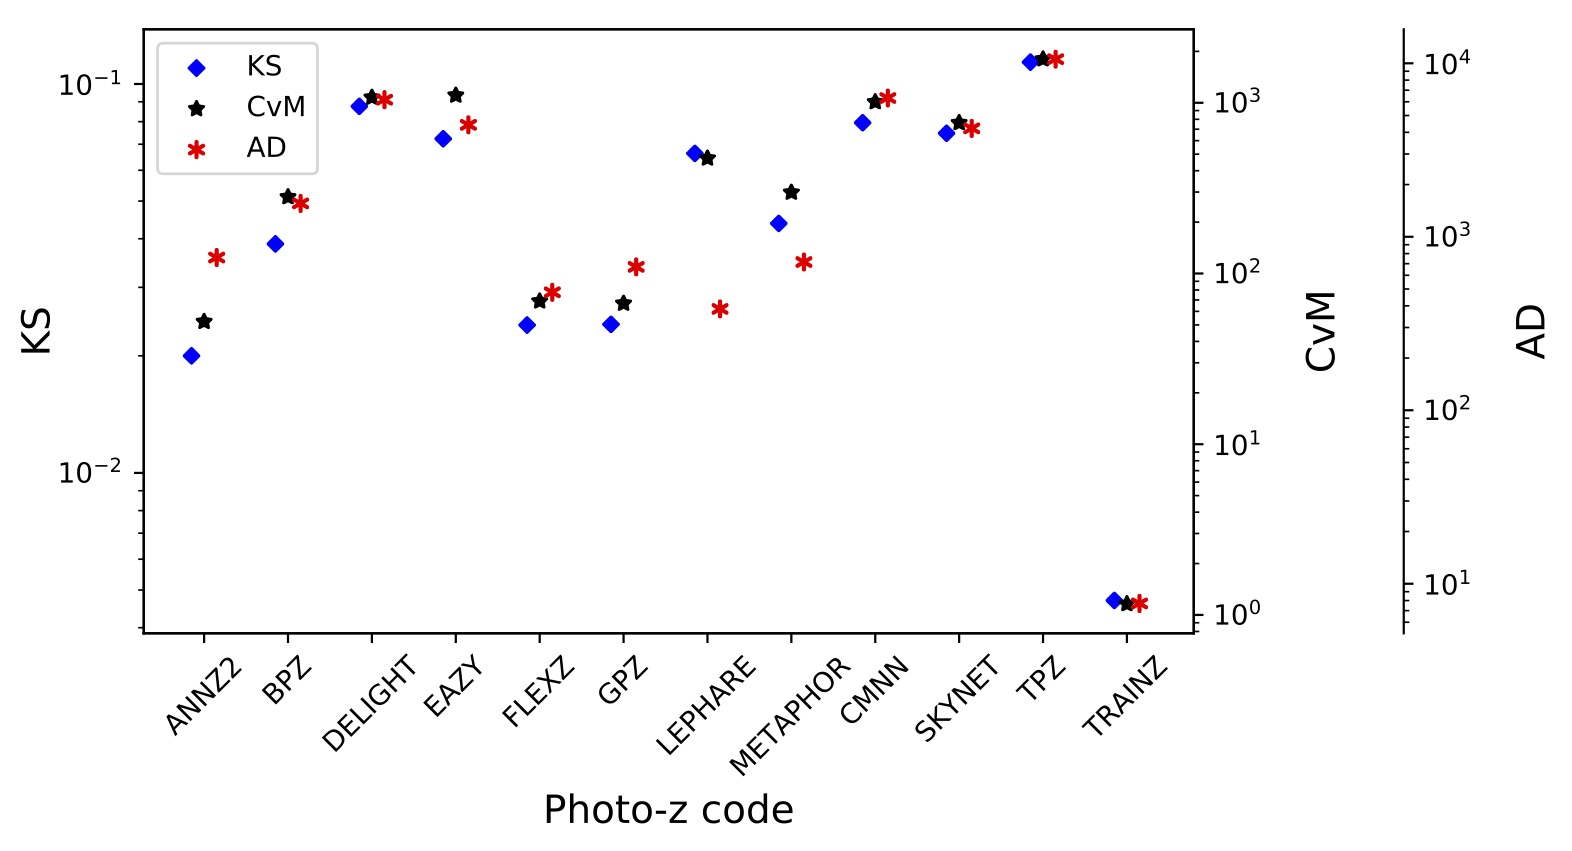
\includegraphics[width=\textwidth]{fig/KSvsCvMvsAD_PIT_withnull_jpg.jpg}
\caption{A visual representation of the Kolmogorov-Smirnoff (KS, blue diamond), Cramer-von Mises (CvM, black star), and Anderson-Darling (AD, red asterisk) statistics for the PIT distributions.  The statistics are often highly correlated, though the AD statistic truncates the extrema of the distribution and can have disparate values compared to KS and CvM.} \label{fig:pit_stats}
\end{figure*}

Fig.~\ref{fig:pit_stats} shows comparative metric values for the quantitative Kolmogorov-Smirnoff (KS), Cramer-Von Mises (CvM), and Anderson Darling (AD) test statistics for each of the codes based on comparing the distribution of their PIT values to the expected uniform distribution over the interval [0,1].  The individual values of the statistic are not as important as the comparative score between the different codes.
%\red{Can p-values be supplied for each statistic? The statistics themselves are difficult to interpret, other than ``lower is better'' (p-value in skgof was broken, having trouble finding 1-sample KS calculation for uniform distribution)}
The AD test statistic diverges for values that include the extrema, and thus is calculated by excluding the edges of the distribution.
We calculate the AD statistic over the range of PIT values $v=[0.01,0.99]$.  \textsc{ANNz2} and \textsc{FlexZBoost} score very well for the PIT metrics.
\textsc{METAPhoR} and \textsc{LePhare} score very well in the PIT AD statistic, but both have a large number of catastrophic outliers, resulting in higher KS and CvM scores.

Given the near-perfect training data, examining the individual codes for explanations for departures from the expected behaviour will be instructive in avoiding similar problems in future tests.
\textsc{ANNz2} performs quite well in $p(z)$ based metrics.  In the specific implementation employed in this paper, the final $p(z)$ is a weighted average of five neural-nets.  During the training process \textsc{ANNz2} compares the percentiles of the redshift training sample against the CDFs of the $p(z)$ sample.  Distributions that more closely match are given extra weight, and the final weights are designed to produce accurate percentiles.  Given that our metrics are focused on the percentile distributions, it is unsurprising that \textsc{ANNz2} performs well in the given metrics.  The discreteness in the individual $p(z)$ estimated by \textsc{ANNz2} can be attributed to the fact that the code was run as a classifier, assigning weights to discrete bins of redshift.  While multiple bins may receive weight, the bins themselves will still be discretized, and no additional smoothing was performed.
Overall, \textsc{FlexZBoost} and \textsc{ANNz2} show the best ensemble agreement in their distribution of PIT values.

\subsection{Metrics of the stacked estimator of the redshift distribution}\label{sec:stackedmetrics}

\begin{figure*}
\centering
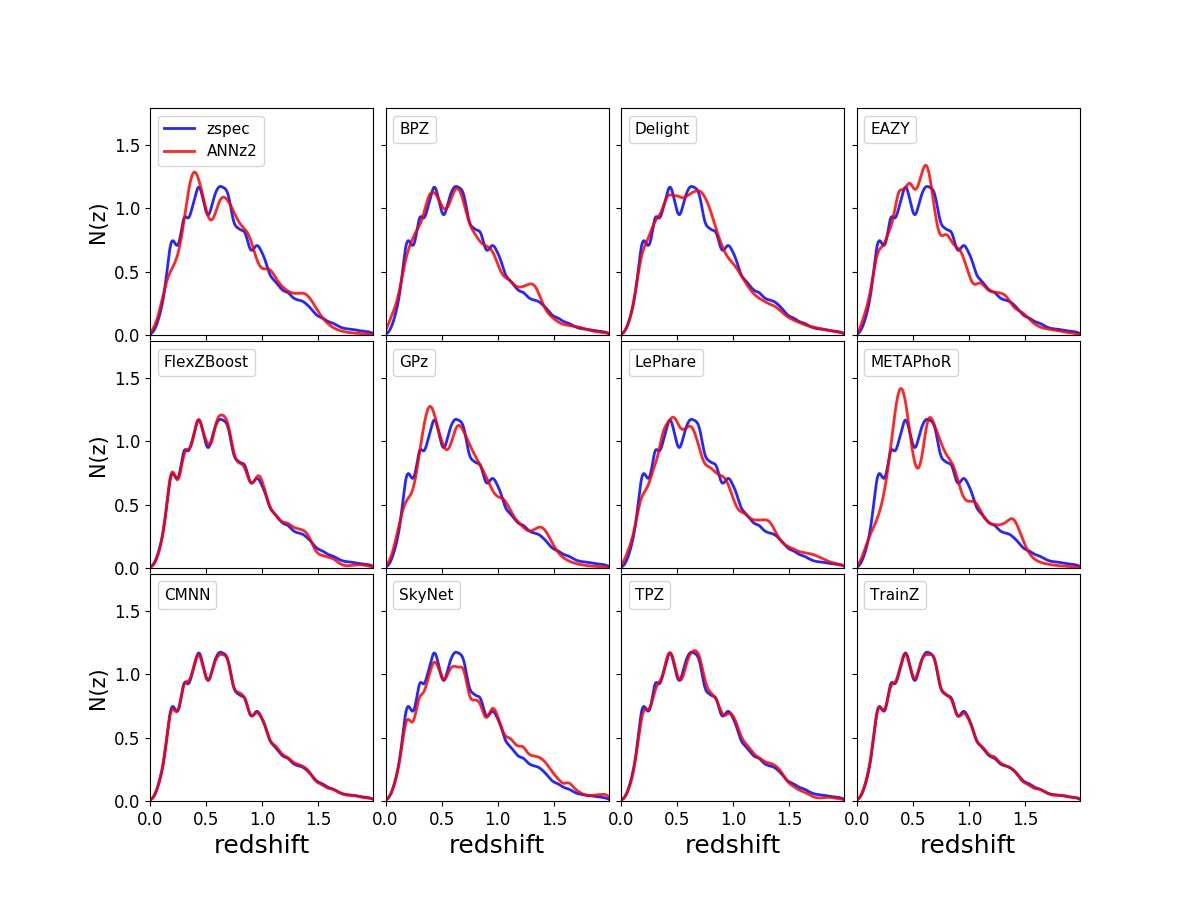
\includegraphics[width=\textwidth]{fig/NZsumplot_12codes_scottsrule.jpg}
\caption{The stacked $p(z)$ produced by each photo-$z$ code ($\hat{N}(z)$, red) compared to the spectroscopic redshift distribution ($N'(z)$, blue).  Varying levels of agreement are seen in the codes.  Both $\hat{N}(z)$ and $N'(z)$ in all codes are smoothed using a single bandwidth chosen via Scott's rule.} \label{fig:nz}
%\aim{Arguably this could also be clarified by showing the true $n'(z)$ once and then differences from it for each cod's stacked estimator\dots}\scc{what if we plot the difference between true and stacked rather than soverposing the two lines? Sam please do not hate me.}
\end{figure*}

\begin{figure*}
\centering
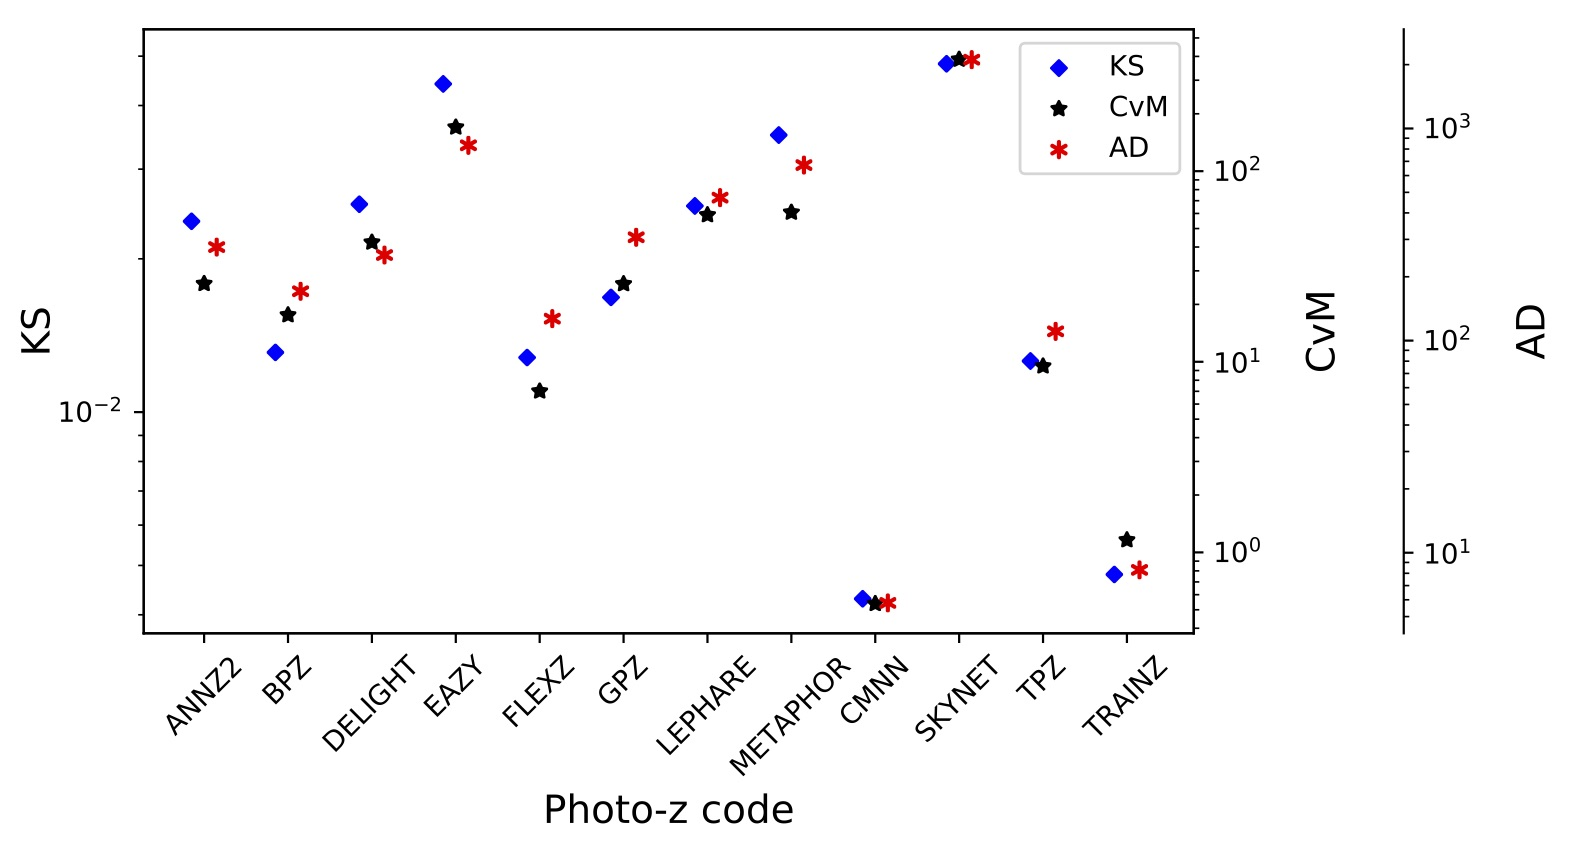
\includegraphics[width=\textwidth]{fig/KSvsCvMvsAD_NZ_withnull_jpg.jpg}
\caption{A visual representation of the Kolmogorov-Smirnoff (KS, blue diamond), Cramer-von Mises (CvM, black star), and Anderson-Darling (AD, red asterisk) statistics for the $\hat{N}(z)$ distributions. The statistics are correlated, the codes with the lowest KS statistics tend to have the lowest CvM and AD statistics.  \textsc{CMNN} performs markedly better than the others in reconstructing the overall $N(z)$ distribution, while \textsc{SkyNet} scores poorly due to an overall bias in its redshift predictions.} \label{fig:nz_stats}
\end{figure*}

Fig.~\ref{fig:nz} shows the stacked $\hat{N}(z)$ distribution compared to the true redshift distribution $N'(z)$ for all tested codes.  The red line indicates the summed $p(z)$ for each code, while the blue line shows the true redshift distribution. All distributions are smoothed via kernel density estimation (KDE) with a common bandwidth chosen via Scott's rule \citep{Scott:1992} in order to minimize differences in small-scale features and make for a more uniform comparison between codes.  While Scott's rule is used to display $N'(z)$ in the figure, all quantitative statistics are computed via the empirical CDF, and are thus unaffected by bandwidth/smoothing choice.
%New text for the new figure
As expected, \textsc{TrainZ} is in excellent agreement with the true redshift distribution: as the training sample is selected from the same underlying distribution as the test set, the redshift distributions are identical, up to Poisson fluctuations due to the finite number of sample galaxies.  \textsc{CMNN} is also in excellent agreement for similar reasons: with a representative training sample of galaxies spanning the colour-space, the sum of the colour-matched neighbour redshifts should return the true redshift distribution. \textsc{FlexZBoost} and \textsc{TPZ} also show very good agreement, with only slight departures, with an over/under-prediction in the high redshift tail of $\hat{N}(z)$ evident around $z\sim1.4$.  In fact, several of the other codes show an excess at $z \sim 1.4$, particularly the template-based codes \textsc{BPZ}, \textsc{EAZY}, and \textsc{LePhare}.  This is likely due to the $4000\ {\rm \AA}$ break passing through the gap between the $z$ and $y$ filters, resulting in a drastic change in $z-y$ colour for galaxies in this redshift range.  With a relative dearth of strong features blue-ward of the $4000\ {\rm \AA}$ break in most galaxy SEDs, the colour change in the two reddest filter bandpasses of a survey has a large influence on the redshift determination.  The $z\sim1.4$ feature is one of the most prominent sources of larger uncertainty in individual galaxy $p(z)$.
In our sample individual galaxy $p(z)$'s tend to be broader around $z\sim1.4$ and point estimates are more uncertain in this regime, as is readily seen in the point-estimate plots shown in Fig.~\ref{fig:pz_pointestimates} and described in the Appendix.  This feature is not unique to this dataset, it is a common occurrence in photo-$z$ estimation.  The fact that similar excesses appear in Figure~\ref{fig:nz} for \textsc{ANNz2} and \textsc{METAPhoR} shows that the effect is not limited to template-based codes.  However, the lack of such a feature in the other codes shows that it is possible to eliminate the degeneracies.  Further study on this issue may provide a solution for codes that suffer from this shortcoming.

%end of new text (and slightly modified text)
Two of the machine learning based codes, \textsc{ANNz2} and \textsc{METAPhoR}, appear to be over-trained, adding excess galaxy probability to the redshift peaks with the largest number of training galaxies, and missing probability in the troughs where training galaxies are of fewer number.
Given that our training data is drawn from the same galaxy population as the test set, and our data has prominent peaks in $N'(z)$, perhaps it is not unexpected that such overtraining occurs in some codes, though the fact that it does not occur in all training-based codes indicates that it may be due to specifics of the implementations of \textsc{ANNz2} and \textsc{METAPhoR}.
A more extensive training/validation set might allow for a better choice of smoothing parameters in individual codes that would avoid such overtraining for these particular codes.
%\aim{Move the text on Scott's Rule to Discussion?}
%Scott's rule \citep{Scott:1992} was used to determine the smoothing bandwidth of the true redshift sample: that is, a single smoothing scale was chosen to represent the true redshift sample for all twelve codes.
%As with the $p(z)$ values in Figure~\ref{fig:pitqq}, different levels of substructure are obvious for the different codes.
%While Scott's rule provides a relatively good general smoothing scale to represent the true $N'(z)$, there are smaller scale fluctuations: while \textsc{FlexZBoost} and \textsc{CMNN} appear somewhat discrepant in Fig.~\ref{fig:nz}, they are actually the two most accurate in terms of their quantitative measurements.
%\textsc{SkyNet} also shows excess small-scale structure, but also shows significant overestimate of the high redshift galaxy population.
\textsc{SkyNet} shows an obvious redshift bias, evident both visually in Figure~\ref{fig:nz} and in the first moment of N(z) listed in Table~\ref{tab:moments}, where it is clearly an outlier.  \textsc{SkyNet} employed a method where a random sample of training galaxies was chosen, but there was no test that the subset was completely representative of the overall redshift distribution.  Unlike the previous implementation of \textsc{SkyNet} in \citet{Bonnett:15}, no effort was made to add extra weight to more rare low and high redshift galaxies.  Either of these decisions could be the cause of the bias seen in our results.  Future runs of \textsc{SkyNet} will explore these implementation choices and their effects.


Figure~\ref{fig:nz_stats} shows the quantitative Kolmogorov-Smirnoff (KS), Cramer-Von Mises (CvM), and Anderson Darling (AD) test statistics for each of the codes for the $\hat{N}(z)$ based measures.
%\red{Can p-values be supplied for each statistic? The statistics themselves are difficult to interpret, other than ``lower is better'' (no, p-values are very difficult to compute for non-uniform distributions)}
\textsc{FlexZBoost}, \textsc{CMNN}, and \textsc{TPZ} outperform the other codes in the $\hat{N}(z)$ metrics.
It is unsurprising that \textsc{CMNN} scores well, as with a near perfectly representative training set means that choosing neighbouring points in color/magnitude space should lead to excellent agreement in the final $\hat{N}(z)$ estimate.  \textsc{TPZ} performed quite poorly in $p(z)$ statistics, but results in a good fit to the overall $N(z)$.  This is somewhat surprising, as performance was optimized for accurate $p(z)$, not $\hat{N}(z)$.  During the validation stage for \textsc{TPZ}, there was a trade off between the width of the $p(z)$ when adjusting a smoothing parameter and overall redshift bias.  The optimal result in the PIT metrics, as illustrated in the shape of the QQ plot, does contain some level of bias as well as a slight underprediction of mean $p(z)$ width, which translates to poor metric scores.  This is something that will be looked into for \textsc{TPZ} in the future.

%\red{discussion of why NN and FZBoost are doing well, how we can try to improve the other codes}
%\textcolor{cyan}{Ann: }


Table~\ref{tab:cdeloss} shows the CDE loss statistic for each photo-$z$ code.  Once again \textsc{FlexZBoost} and \textsc{CMNN} score very well for the stacked $\hat{N}(z)$ metrics, as do \textsc{GPz} and \textsc{TPZ}.  The CDE loss measures how well individual PDFs are estimated, and codes with a low CDE loss tend to have good $\hat{N}(z)$ estimates (though the reverse is not necessarily true). \textsc{FlexZBoost} is optimized to minimize CDE loss which may explain why the method has good ensemble metrics as well. Note from Table~\ref{tab:cdeloss} that both \textsc{FlexZBoost} and \textsc{CMNN} have low CDE losses.  Empirically, we have found that PIT RMSE is not as closely correlated to CDE loss as it is to the $N(z)$ statistics.  As CDE loss is a better measure of individual redshift performance, rather than ensemble distribution performance, this statistic is a better indicator of which codes will be most likely to perform well for science cases where single objects are employed.

Table~\ref{tab:rmse} gives the root-mean-square-error (RMSE) statistics for both the PIT and N(z) estimators.  The PIT value calculates the RMSE between the quantiles shown in the QQ plot in Figure~\ref{fig:pitqq} and the diagonal, while the N(z) calculates the RMSE between the cumulative distribution of the stacked $\hat{N}(z)$ and the true redshift distribution $N'(z)$.  %\red{more about RMSE?  Or remove it? It's barely described in Section~\ref{sec:metrics} and wasn't even referred to in the text until I added this on June 29th--SJS.}

Table~\ref{tab:moments} lists the first three moments of the stacked $\hat{N}(z)$ distribution, including the moments of the ``truth'' distribution for comparison.  Several codes are able to reproduce the mean and variance of the distribution to less than a per cent, while several codes do not, which may be a cause for concern, given that mean and variance of the redshift distribution are key properties in cosmological analyses.  We note that this stated goal of the study as defined for participants was to accurately reproduce $p(z)$, the ``stacking'' of the probability distributions to estimate $\hat{N}(z)$ was not the focus as stated to the participants.  This explains why some of the best-performing empirical codes in terms of $p(z)$ measures (e.~g.~\textsc{FlexZBoost}) do not do as well at reproducing $\hat{N}(z)$ moments.  Had we defined a different parameter to optimize, in this case overall accuracy of $\hat{N}(z)$ rather than individual $p(z)$, would result in improved performance in a particular metric.  That is, optimizing photo-$z$ performance for one metric does not automatically give optimal performance for other metrics.  As previously stated, there are a variety of scientific use cases for photo-$z$'s in large upcoming surveys, and care must be taken in how the metrics used to optimize catalog photometric redshifts are defined as well as in how they are used.  In addition, very few scientific use cases will employ the overall $\hat{N}(z)$ with no cuts, as we explore in this paper.  We discuss more realistic tomographic bin selections that will be explored in a follow-up paper in Section~\ref{sec:futurework}.
%\red{[mention that we are calculating moments for the entire sample, will look at fiducial tomographic bins in a follow-up paper (unless group and reviewers realy think we should include in this paper.]}
%\red{FlexZBoost has some of the best $n(z)$ statistics, but the moments are not good.  Why is this?  Is it the over/underprediction of the high redshift part of the distribution?  Discuss this after talking with Rafael.}

%\subsection{Response of Individual Codes}
%\label{sec:res:pz_indiv_codes}
%\red{this may be incorporated in to 5.1 and 5.2 rather than live in its own section!}


%\red{HOW CODES deal with negative fluxes, and magnitude uncertainties}

%\red{overall conclusions of the Results section}

\subsection{Interpretation of metrics}\label{sec:caution}
%Caution on metrics and photo-$z$ codes}\label{sec:caution}
%(Alex Malz, Sam Schmidt)

Samples from accurate photo-$z$ posteriors should reproduce the space of $p(z, data)$. However, it is difficult to test this reconstruction given our data set, as the galaxy distributions arise from mock objects pasted on to an underlying dark matter halo catalogue with properties designed to match empirical relations, rather than being drawn from statistical distributions in redshift.  In previous sections we have mentioned that optimizing for a specific metric does not guarantee good performance on other metrics, nor is there any guarantee that good performance by our metrics corresponds to \textit{accurate} photo-$z$ posteriors.
%\aim{Explain that samples from accurate photo-$z$ posteriors should reconstruct the space of $p(z, data)$, a test we can't check with our datasets.}
In other words, we can construct photo-$z$ estimators that provide good coverage in many of our tests, but which have very little predictive power.


The \trainz\ estimator, which assigns every galaxy a $p(z)$ equal to $N(z)$ of the training set as described in Section~\ref{sec:method:trainz}, is introduced as a ``null test'' to demonstrate this point via \textit{reductio ad absurdum}.
\trainz\ outperforms all codes on the PIT-based metrics, and all but one code on the $N(z)$ based statistics.
Because our training set is perfectly representative of the test set, $N(z)$ should be identical for both sets down to statistical noise.
%\textit{Explain the connection between \trainz\ and these metrics.}

The CDE loss and point estimate metrics, however, successfully identify problems with \trainz.
As shown in Appendix~\ref{sec:pointmetrics}, \trainz has identical $ZPEAK$ and $ZWEIGHT$ values for every galaxy, and thus the photo-$z$s are constant as a function of spec-$z$s, i.e. a horizontal line at the mode and mean of the training set distribution respectively.  The explicit dependence on the \it{individual} posteriors in the calculation of the CDE loss, described in Section~\ref{sec:CDE_loss}, distinguishes this metric from the other $p(z)$ metrics that test the overall ensemble of $p(z)$ distributions.  With a representative training set, \trainz\ will score well on the ensemble metrics, but fails miserably for metrics tied to individual redshifts.  We note that many of the ensemble-based metrics are prominent in the photo-$z$ literature despite their inability to identify problems such as those exemplified by \trainz.

%\aim{Explain why CDE loss is different from other metrics (isn't fooled by \trainz) and note that the others have more of a presence in the literature despite their flaw of failing to identify this severe problem.}

% While looking at one, or even most of our metrics would have given the impression that this estimator was nearly optimal, red flags in CDE loss and point estimates reveal the problems.
%[more caution on over-reliance on metrics, and making sure that metrics test all of what you want] \red{this definitely still needs work}
In summary, context is crucial to interpreting metrics and defending against the likes of \trainz.
The best photo-$z$ method is the one that most effectively achieves our science goals, not the one that performs best on a metric that does not accurately reflect those goals.
In the absence of clear goals or the information necessary for a principled metric definition, we must think carefully before choosing a single metric

%\begin{table*}  %%% DATA TABLE %%%
%\caption{KS, CvM and AD statistics for each photo-$z$ code.} \label{tab:results}
%PIT statistic
%
%\begin{tabular}{lrrrr}
%\hline
%\bf Photo-$z$ Code & \bf KS & \bf CvM & \bf AD & \bf AD \\
%                   &        &         & $v=[0.05,0.95]$ & $v=[0.01,0.99]$        \\
%\hline
%\textsc{ANNz2} 		& $0.0200$ &   $52.25$ &   $583.0$ &   $759.2$ \\
%\textsc{BPZ} 		& $0.0388$ &  $280.79$ &  $1361.4$ &  $1557.5$ \\
%%\textsc{Delight} 	& $0.1380$ & $3040.59$ & $13880.2$ & $17761.4$ \\
%\textsc{Delight}    & $0.0876$ & $1075.17$ & $4407.8$  & $6167.5$\\
%%\textsc{EAZY} 		& $0.0690$ &  $994.19$ &  $3479.5$ &  $4158.8$ \\
%\textsc{EAZY}       & $0.0723$ & $1105.58$ & $3475.0$  & $4418.6$\\
%%\textsc{FlexZBoost} & $0.0260$ &   $70.58$ &   $595.0$ &   $533.0$ \\
%\textsc{FlexZBoost} & $0.0240$ &   $68.83$ &   $567.9$ &   $478.8$\\
%\textsc{GPz} 		& $0.0449$ &  $258.56$ &   $904.8$ &  $1414.8$ \\
%\textsc{LePhare} 	& $0.0663$ &  $473.05$ &    $85.9$ &   $383.8$ \\
%\textsc{METAPhoR} 	& $0.0438$ &  $298.56$ &   $248.6$ &   $715.5$ \\
%%\textsc{CMNN} 		& $-$ & $-$ & $-$ & $-$ \\
%\textsc{CMNN}         & $0.0795$  &$1011.11$ &  $3908.2$ &  $6307.5$ \\
%\textsc{SkyNet} 	& $0.0747$ &  $763.00$ &  $2740.2$ &  $4216.4$ \\
%\textsc{TPZ} 		& $0.1138$ & $1801.74$ &  $9046.2$ & $10565.7$ \\
%%\textsc{Frankenz}	& $-$ & $-$ & $-$ & $-$ \\
%\hline
%\end{tabular}

%Stacked $n(z)$ statistic
%
%\begin{tabular}{lrrrr}
%\hline
%\bf Photo-$z$ Code & \bf KS & \bf CvM & \bf AD & \bf AD \\
%                   &        &         & $z=[0.002,2.0]$ & $z=[0.0,2.0]$        \\
%\hline
%\textsc{ANNz2} 		& $0.0237$ &  $25.676$ &   $276.4$ &   $276.0$ \\
%\textsc{BPZ} 		& $0.0131$ &  $17.587$ &   $169.0$ &   $170.9$ \\
%%\textsc{Delight} 	& $0.0184$ &  $18.975$ &   $151.5$ &   $151.5$ \\
%\textsc{Delight}    & $0.0256$ &  $42.341$ &   $253.3$ &   $253.2$ \\
%%\textsc{EAZY} 		& $0.0434$ & $167.329$ &   $811.3$ &   $817.0$ \\
%\textsc{EAZY}       & $0.0441$ & $169.977$ &   $827.7$ &   $833.3$ \\
%%\textsc{FlexZBoost} & $0.0065$ &   $2.764$ &    $24.7$ &    $24.6$ \\
%\textsc{FlexZBoost} & $0.0128$ &   $7.007$ &  $127.02$ &   $126.9$\\
%\textsc{GPz} 		& $0.0168$ &  $25.605$ &   $307.1$ &   $307.1$ \\
%\textsc{LePhare} 	& $0.0254$ &  $58.900$ &   $477.4$ &   $472.0$ \\
%\textsc{METAPhoR} 	& $0.0350$ &  $60.790$ &   $671.9$ &   $672.3$ \\
%%\textsc{CMNN} 		& $-$ & $-$ & $-$ & $-$ \\
%\textsc{CMNN}         & $0.0043$ & $0.538$   &   $5.6$   &      $5.8$ \\
%\textsc{SkyNet} 	& $0.0483$ & $385.830$ &  $2119.4$ &  $2110.3$ \\
%\textsc{TPZ} 		& $0.0126$ &   $9.483$ &   $110.7$ &   $110.6$ \\
%%\textsc{Frankenz}	& $-$ & $-$ & $-$ & $-$ \\
%\hline
%\end{tabular}
%\end{table*}

\begin{table}  %%% DATA TABLE %%%
\centering
\caption{CDE loss statistic for each photo-$z$ code.} \label{tab:cdeloss}
\begin{tabular}{lr}
\hline
\bf Photo-$z$ Code & \bf CDE Loss \\
\hline
\textsc{ANNz2} 		& $-6.88$ \\
\textsc{BPZ} 		& $-7.82$ \\
%\textsc{Delight} 	& $-4.06$ \\
\textsc{Delight}    & $-8.33$\\
%\textsc{EAZY} 		& $-7.97$ \\
\textsc{EAZY}       & $-7.07$ \\
%\textsc{FlexZBoost} & $-11.51$ \\
\textsc{FlexZBoost} & $-10.60$\\
\textsc{GPz} 		& $-9.93$ \\
\textsc{LePhare} 	& $-1.66$ \\
\textsc{METAPhoR} 	& $-6.28$ \\
%\textsc{CMNN} 		& $-$ \\
\textsc{CMNN}         & $-10.43$ \\
\textsc{SkyNet} 	& $-7.89$ \\
\textsc{TPZ} 		& $-9.55$ \\
\hline
\trainz		& $-0.83$ \\
%\textsc{Frankenz}	& $-$  \\
%\hline
\end{tabular}
\end{table}

\begin{table}
\setlength{\tabcolsep}{2pt}
\begin{center}
\caption{Root-Mean-Square-Error (RMSE) statistics for the twelve photo-z codes for both PIT and $\hat{N}(z)$ distributions.}\label{tab:rmse}
\begin{tabular}{lcc}
\hline
\hline
Root-Mean-Square-Error \\
(RMSE) statistics \\
\hline
Photo-z Code & PIT RMSE & N(z) RMSE\\
\hline
\textsc{ANNz2}      & 0.019 & 0.0054\\
\textsc{BPZ}        & 0.032 & 0.0050\\
\textsc{Delight}    & 0.111 & 0.0056\\
\textsc{EAZY}       & 0.054 & 0.0102\\
\textsc{FlexZBoost} & 0.021 & 0.0022\\
\textsc{GPz}        & 0.027 & 0.0042\\
\textsc{LePhare}    & 0.028 & 0.0062\\
\textsc{METAPhoR}   & 0.064 & 0.0081\\
\textsc{CMNN}         & 0.108 & 0.0009\\
\textsc{Skynet}     & 0.054 & 0.0144\\
\textsc{TPZ}        & 0.082 & 0.0031\\
\hline
\trainz		& 0.0025 & 0.0013\\
\end{tabular}
\end{center}
\end{table}

%\begin{table}
%\begin{center}
%caption{RMSE Statistics for the 11 Photo-z codes for DC1 $i<25.3$ ``gold'' sample}\label{tab:pitrmse}
%%\begin{tabular}{|l|c|c|c|c|}
%\begin{tabular}{lc}
%\hline
%\hline
% PIT RMSE statistics \\
%\hline
%Photo-z Code & PIT RMSE\\
%\hline
%\texttt{ANNz2}      & 0.019\\
%\texttt{BPZ}        & 0.032\\
%\texttt{Delight}    & 0.111\\
%\texttt{EAZY}       & 0.054\\
%\texttt{FlexZBoost} & 0.021\\
%\texttt{GPz}        & 0.048\\
%texttt{LePhare}    & 0.028\\
%\texttt{METAPhoR}   & 0.064\\
%\texttt{NN}         & 0.108 \\
%\texttt{Skynet}     & 0.054\\
%texttt{TPZ}        & 0.082\\
%\hline
%\end{tabular}
%\end{center}
%\end{table}
%
%\begin{table}
%\begin{center}
%\caption{RMSE Statistics for the 11 Photo-z codes for DC1 $i<25.3$ ``gold'' sample}\label{tab:nzrmse}
%%\begin{tabular}{|l|c|c|c|c|}
%\begin{tabular}{lc}
%\hline
%\hline
% N(z) RMSE statistics \\
%\hline
%hoto-z Code & N(z) RMSE\\
%\hline
%\texttt{ANNz2}      & 0.0054\\
%\texttt{BPZ}        & 0.0050\\
%\texttt{Delight}    & 0.0056\\
%\texttt{EAZY}       & 0.0102\\
%\texttt{FlexZBoost} & 0.0022\\
%\texttt{GPz}        & 0.0042\\
%\texttt{LePhare}    & 0.0062\\
%\texttt{METAPhoR}   & 0.0081\\
%\texttt{NN}         & 0.0009\\
%\texttt{Skynet}     & 0.0144\\
%\texttt{TPZ}        & 0.0031\\
%\end{tabular}
%\end{center}
%\end{table}

\begin{table}
\setlength{\tabcolsep}{2pt}
\caption{Moments of the stacked $\hat{N}(z)$ distribution}\label{tab:moments}
\begin{tabular}{lccc}
\hline
\hline
 \multicolumn{4}{l}{Stacked $n(z)$ Moments} \\
\hline
              & 1st Moment & 2nd Moment & 3rd Moment \\
\textsc{Truth}     & 0.701      &   0.630    & 0.671  \\
\hline
Photo-z Code       & 1st Moment & 2nd Moment & 3rd Moment\\
\hline
\textsc{ANNz2}     & 0.702      & 0.625      & 0.653    \\
\textsc{BPZ}       & 0.699      & 0.629      & 0.671    \\
\textsc{Delight}   & 0.692      & 0.609      & 0.638    \\
\textsc{EAZY}      & 0.681      & 0.595      & 0.619    \\
\textsc{FlexZBoost}& 0.694      & 0.610      & 0.631    \\
\textsc{GPz}       & 0.696      & 0.615      & 0.639    \\
\textsc{LePhare}   & 0.718      & 0.668      & 0.741    \\
\textsc{METAPhoR}  & 0.705      & 0.628      & 0.657    \\
\textsc{CMNN}        & 0.701      & 0.628      & 0.667    \\
\textsc{Skynet}    & 0.743      & 0.708      & 0.797    \\
\textsc{TPZ}       & 0.700      & 0.619      & 0.643    \\
\hline
\trainz	   & 0.699 		& 0.627 	& 0.666 \\
\end{tabular}
\end{table}
